\documentclass[UTF8]{article}
\usepackage{ctex}
\usepackage{geometry}
\usepackage{cite}
\usepackage{tikz}
\usepackage{xcolor}
\usepackage{listings}
\usepackage{graphicx}
\usetikzlibrary{graphs, positioning, quotes, shapes.geometric}
\usepackage{url}
\usepackage{threeparttable}
%\usepackage{CJK}
\usepackage[colorlinks,
linkcolor=blue,
anchorcolor=blue, 
citecolor=blue,        
]{hyperref}
\usepackage{subfigure}
\usepackage[graphicx]{realboxes}
%\ctexset{bibname=}
\geometry{top=1cm}
\begin{document}
	\title{\vspace{+10pt} \heiti \textbf {智能水务分析模型}}
	\songti
	\author{oneboyi}
	\date{}
	\maketitle  
	\section*{\centering{摘要}}
		\songti anchorc
		\\ \heiti 关键词:\songti IQR、非正态分布、箱线图、孤立森林
		\newpage
	\section{问题重述}
		\subsection{问题背景}
		\par 供水系统在我们的日程生活中至关重要,但是供水系统有时会发生各种各样的故障,从而导致漏水的发生,这是一个大问题。在这样的背景下,电磁流量计应运而生,用于测量流量以及监测漏水,一种方法是获取某一区域输入和输出水流量的插值加以评价。 
		\par 如今已经有许多基于流量数据的分析方法,但是还有一些挑战存在,比较重要的三个:首先是需要设计一个通用模型来了解流量计的数据模式,然后是如何更加快速地检测流量异常,最后一个挑战是如何应对噪声的影响。\cite[C1]{znswxxh}
		\subsection{具体问题}
		\par 您的团队需要设计一个模型来应对上述挑战,需要对给定数据进行清理,开发异常检测模型,并优化模型,数据是八个不同虚拟区域的输入水流量和输出水流量之差。具体的任务有:

		\begin{itemize}
			\item 分析数据模式,建立检测异常的标准
			\item 建立通用模型对八个区域进行异常值检测
			\item 测试模型并解释建模和异常值检测的结果
		\end{itemize}
		ok
	\section{数据模式分析与异常检测标准的确立}	
	\subsection{数据概览分析}
		\par 题目所给的数据来自于八个不同的虚拟地区,每个地区的流量差值是一个与时间相关的变量,这些值中既有正数,也有负数。大部分流量之差的绝对值都在10以内,如果发现绝对值过大,则可初步认为该数据是异常数据。流量数据随着时间的变化而变化,不同地区流量数据随时间变化的规律也各不相同。
		\par 首先判断各个地区的数据是否满足正态分布,采用四分位距的方法判断是否满足或者接近于正太分布,如果符合正态分布,则可以使用Z-score判断数据是否异常,如果不符合,则需要考虑其他的方法。
		\par 计算可得八个虚拟地区输入和输出水流量之差的四分位距:
		\begin{table}[!ht]
    \centering
	\resizebox{0.8\textwidth}{!}
	{
    \begin{tabular}{|l|l|l|l|l|l|l|l|l|}
    \hline
        region\_1 & region\_2 & region\_3 & region\_4 & region\_5 & region\_6 & region\_7 & region\_8 \\ \hline
        3.802019768 & 1.108408668 & 1.2881612 & 0.678413944 & 4.157332959 & 4.746437346 & 6.514955518 & 1.616935081 \\ \hline
    \end{tabular}
	}
	\end{table}
	\\可见并不满足正态分布的要求,因此不能采用Z-score判断数据是否异常。对于不满足正态分布的数据,可以使用箱线图进行异常数据的检测。
	\subsection{利用箱线图进行数据分析并检测异常数据}
	下面是根据八个地区数据所作出的箱线图\ref{Box},可以初步比较直观地对数据进行分析,也可以看出哪些是异常数据:
\begin{figure}[!h]
\centering %表示居中
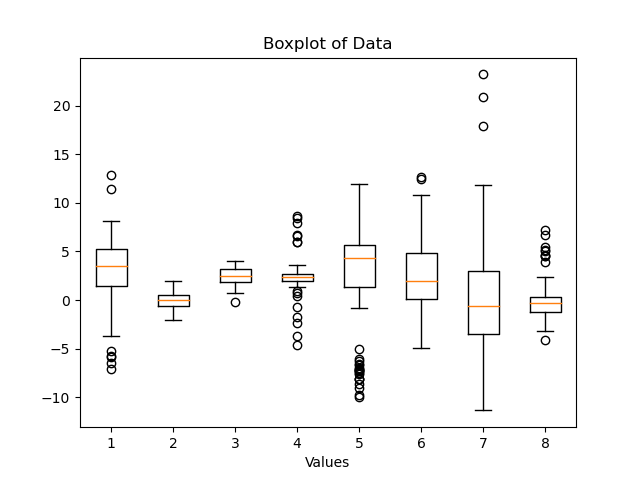
\includegraphics[height=4.5cm,width=9.5cm]{pictures/BoxPlot.png}
% [height=4.5cm]表示高度
%[width=9.5cm]表示宽度
%{111.eps}表示eps格式的图片,名为111
\caption{八个虚拟地区的箱线图}
%图片的名称
\label{Box}
%图片的标签,用于文章中的引用,注意到标签的数字与实际文章显示的数字可能不同
\end{figure}
	\section{建立检测异常的标准}
	\subsection{}
	\section{模型假设}
		anch
	\begin{itemize}
		\item 在经济建设中,主要由劳动人口作出贡献,因此用劳动人口数量和劳动人口的占比这两组变量来概括劳动人口规模
		\item 经济发展起点由前一年国内生产总值决定,资源禀赋由耕地面积和工业企业数量决定,教育水平由教育经费、教育的普及率、入学率和毕业生人数等决定
		\item 多重共线性检验后得到的模型,如果其在改进后依然存在严重的多重共线性,则进一步深入分析该模型,判断能不能忽略多重共线性对其的影响
		\item 该经济增长的回归模型是正确设定的
		\item 所有自变量的随机误差项满足正态分布且均值为0,且与相应自变量同方差、不序列相关
	\end{itemize}
	\section{模型主要变量符号及含义}
		\begin{center}
			\begin{threeparttable}
				\setlength{\tabcolsep}{10mm}
				\begin{tabular}{ccc}
				\hline
				序号 & 符号 & 意义\\
				\hline
				1 & Y1 & 国内生产总值\\
				2 & Y2 & 人均国内生产总值\\
				3 & Y3 & 人均国内生产总值增长率\\
				4 & X1 & 实际利用外商直接投资金额\\
				5 & X2 & 年度资源禀赋\\
				6 & X3 & 年度教育水平\\
				7 & X4 & 年度劳动人口规模\\
				8 & X5 & 该年经济发展起点\\
				9 & X6 & 虚拟变量A1\tnote{1}\\
				10 & X7 & 虚拟变量A2\tnote{2}\\
				11 & t & 年份\\
				\hline
				\end{tabular}
				\begin{tablenotes}
					\item [1] 当年无疫情影响经济增长
					\item [2] 当年有疫情影响经济增长
				\end{tablenotes}
			\end{threeparttable}
		\end{center}
		hehe
	\section{模型建立}
		a
	\section{模型的检验与修正}
		对
	\section{模型求解}
		dui
	\section{模型评价}
		hao
	\bibliographystyle{unsrt}
	\bibliography{refs.bib}
	\section*{附录}
	\subsection*{I 程序源代码}
		hehe
	\subsection*{II 支撑材料文件列表}
		hehe
	\begin{itemize}
		\item 分类原始数据.rar
		\item 原始数据汇总.xls
		\item 建模求解分析过程草稿.docx
		\item 数据处理过程,结果及代码.docx
	\end{itemize}
\end{document}